\section{Churn Probability Prediction}
\label{sec:prediction}

A key benefit of our model is that the parameters inferred from data (called training data) can be reused to make prediction on new data. This is process 5.2 in the modelling pipeline (\Cref{tab:pipeline}) proposed in section \ref{sec:modelPipeline}. The potential concern in practice is model overfitting, namely that the model parameters ($\theta$, clusters, states) correspond too closely to the training data, and mail fail to fit additional data or predict reliably. We will investigate on overfitting issue.

\subsection{Prediction Workflow}

We summarise the the prediction workflow in the schematic \Cref{fig:predictionWorkflow}.

\begin{figure}[!h]
\centering
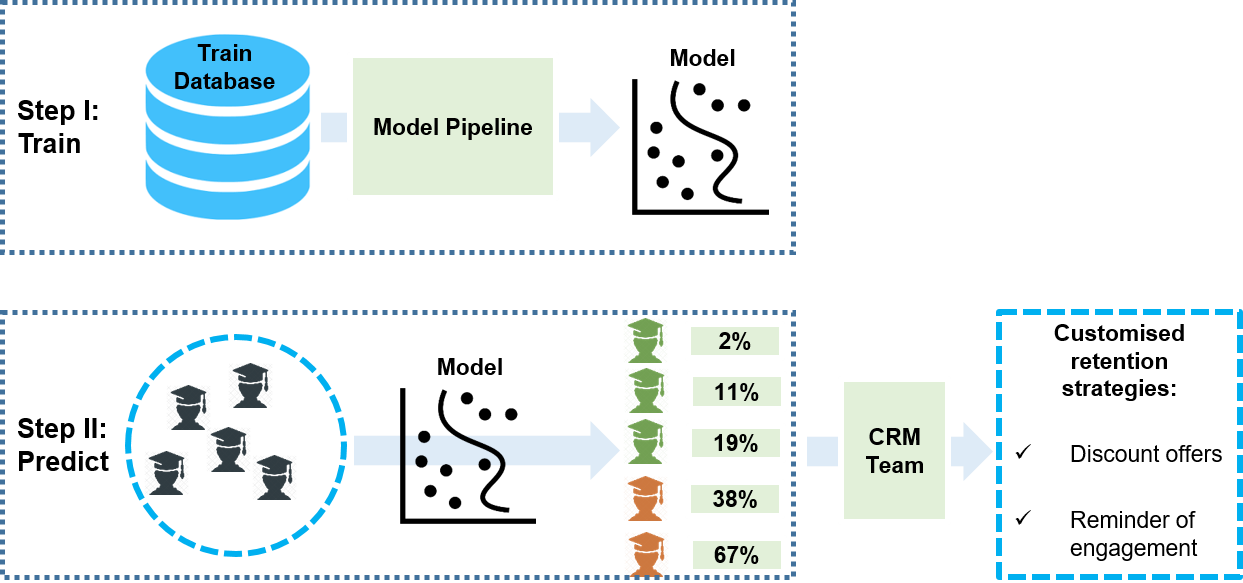
\includegraphics[scale=0.7]{PredictionWorkflow.png}
\caption{Prediction workflow in two steps, and its downstream process.}
\label{fig:predictionWorkflow}
\end{figure}

In the train step, we need select data of proper pupils to feed into the model. Proper pupils means that the pupils must have already churned in history, otherwise we do not know the churn outcome and cannot capture the whole behavioural path. The data trimming is discussed in section \ref{sec:dataScope}. The model we will obtain at the end of train step is parametrised by
\begin{itemize}
\item a collection of parameters $\{ a_i, b_i, \lambda_i, x_i^\text{min}, x_i^\text{max}\}_{i=1}^m$ for transformation and standardisation of feature data;
\item a posterior distribution $\mathbb{P} (\theta | \mathbf{X}, \alpha, G_0)$ guiding observation-to-cluster assignment, and cluster-associated churn risk; and
\item a definition of a finite set of states guiding cluster-to-state assignment.
\end{itemize}
The model can be used in the predict step to map from a pupil's feature data to a state assignment as well as an estimated churn probability. Moreover, we can locate the relative level of the pupil's features in the population distribution, thus figuring out the possible reasons for the resulting churn risk.

An important note is that our model is trained on pupils' monthly-aggregated behaviours, such as total time spent in using the service, the average marks obtained, etc. Hence, the prediction shall only be made on monthly-aggregated behaviour data. This seems contradict to prediction task, since we do not want to predict the churn risk on the last day of the current prediction when the churn outcome has already been or will be immediately known. A suggested remedy is to aggregate behaviours on calendar month for prediction task. For example, suppose on 2018-06-20, we would like to assess the churn risk for a pupil whose current subscription will expire on 2018-06-30. Then we can collect its behaviours from 2018-5-19 to 2018-06-19 and feed into the model to make prediction. This remedy, however, assumes the pupil has at least had renewed his subscription once. In the case where the pupil is a new joiner, we can scale his 20-day behaviours to 30-day behaviours as a proxy. For example, if he has spent 30 hours in using the service for 20 days, we can assume he will spend 45 hours for this customer month.

\subsection{Evaluating Overfitting}

To investigate the overfitting issue, we split the data into train set and test set, and train the model using train data set, then compare the churn probability assignments for train set and test set.

\begin{figure}[!h]
\centering
	\subfloat[Train Pct = 5\%]{%
		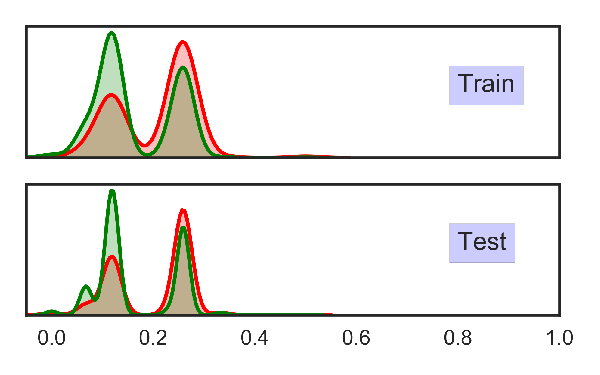
\includegraphics[scale=.7]{Overfitting005.pdf}
	}
	\subfloat[Train Pct = 10\%]{%
		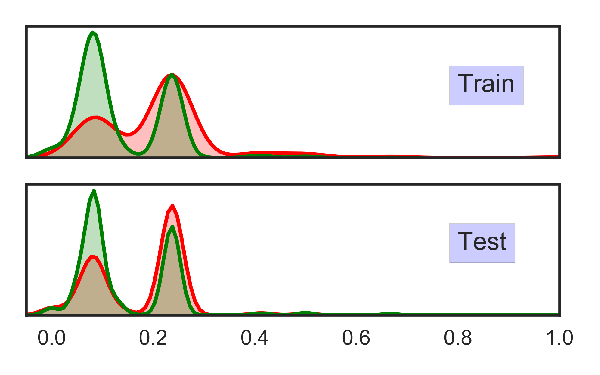
\includegraphics[scale=.7]{Overfitting010.pdf}
	}
	\hspace{0mm}
	\subfloat[Train Pct = 50\%]{%
		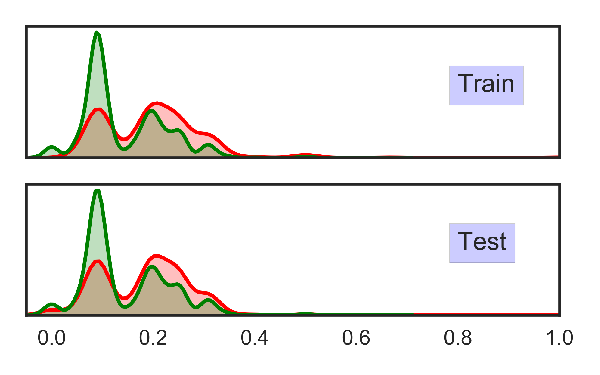
\includegraphics[scale=.7]{Overfitting050.pdf}
	}
	\subfloat[Train Pct = 70\%]{%
		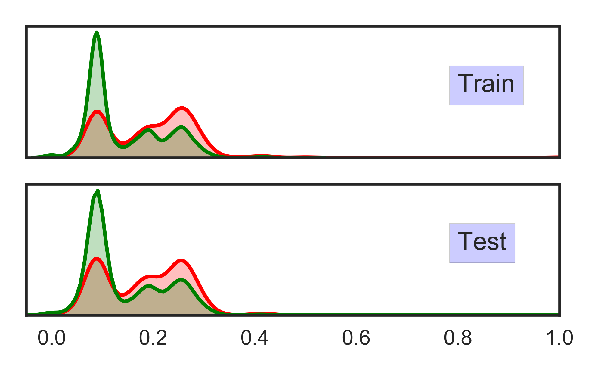
\includegraphics[scale=.7]{Overfitting070.pdf}
	}
	\hspace{0mm}
	\subfloat[Train Pct = 90\%]{%
		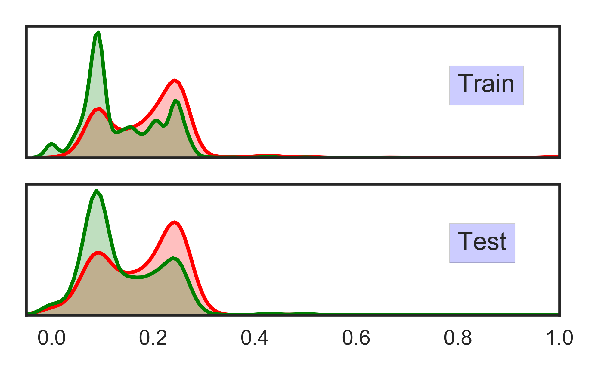
\includegraphics[scale=.7]{Overfitting090.pdf}
	}
	\subfloat[Train Pct = 95\%]{%
		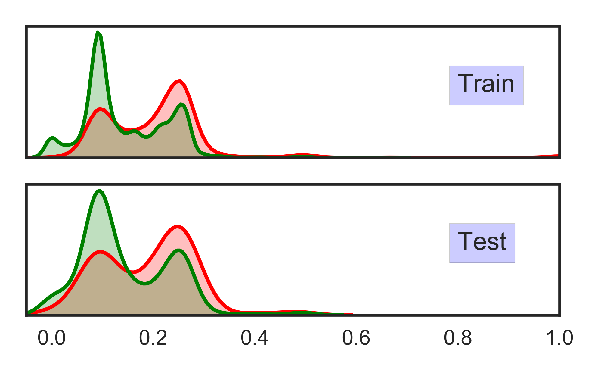
\includegraphics[scale=.7]{Overfitting095.pdf}
	}
\caption{Distributions of computed churn probabilities for churner (red) and non-churner (green) in both train and test data sets, given different proportions of data trained.}
\label{eq:overfitting}
\end{figure}

The splitting is random. We compare the distributions of computed churn probabilities for churner and non-churner in both train and test data sets, given different proportions of data trained. When the proportion of train data set is small (5\%, 10\%), distributions inferred from both sets appear not similar. However, when there is very large train data set, distributions inferred from train and test sets appear very similar. It seems larger data set for training is preferred and the overfitting issue is not significant. A possible explanation is that in our model, the clustering task is performed without knowing any churn outcome information, so that there is not a ``fitting'' process involved when do clustering. Moreover, since it is mixture-based, more data mean statistically the estimated model parameters will be closer to their true value.